\appendix
\renewcommand{\thesection}{APPENDIX \Alph{section}}

\section{ - Nem-relativisztikus közelítés} \label{appendix:A}

\section{ - Ábrák} \label{appendix:B}
\topskip0pt
\vspace*{\fill}
\begin{center}
    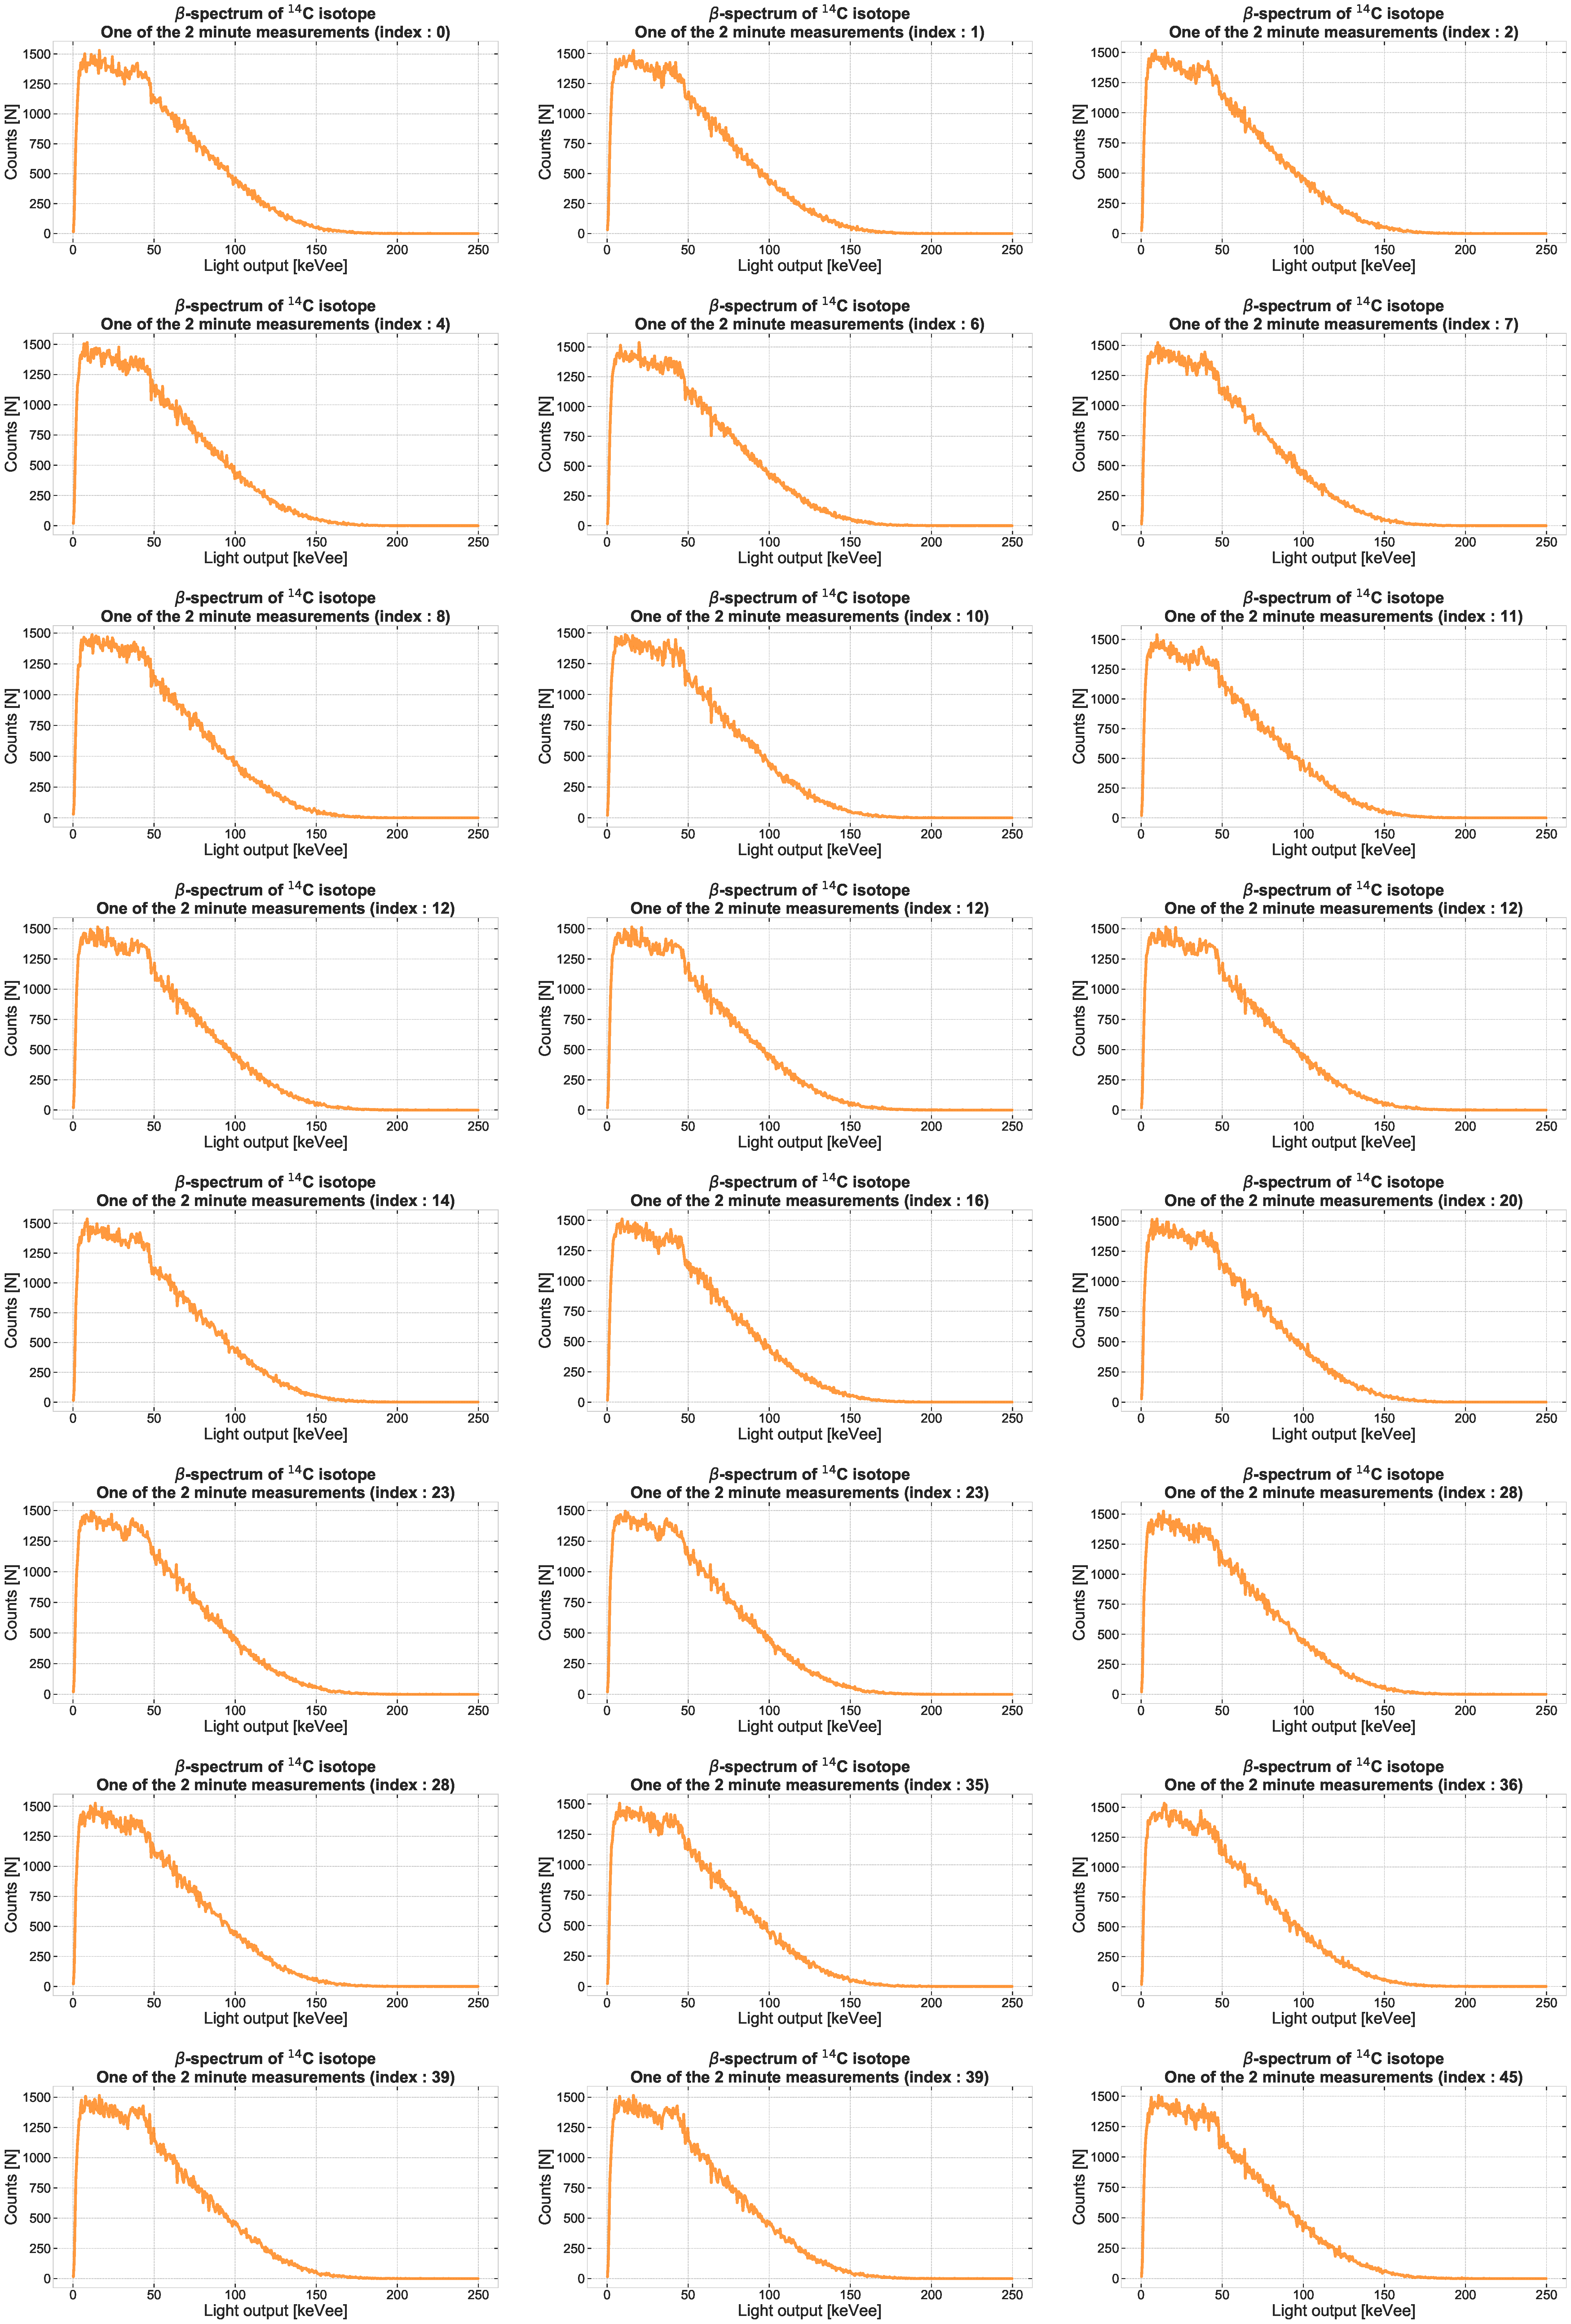
\includegraphics[width=\textwidth]{random_spectrums.pdf}
    \captionof{figure}{Az általunk vizsgált $^{14}$C különböző, egymás utáni 2 perces mérésekből származó $\beta$-spektrumai. Az összes 49 sikeres mérés közül 12 darab van az ábrára véletlenszerűen kiválasztva.} \label{fig:1}
\end{center}
\begin{center}
    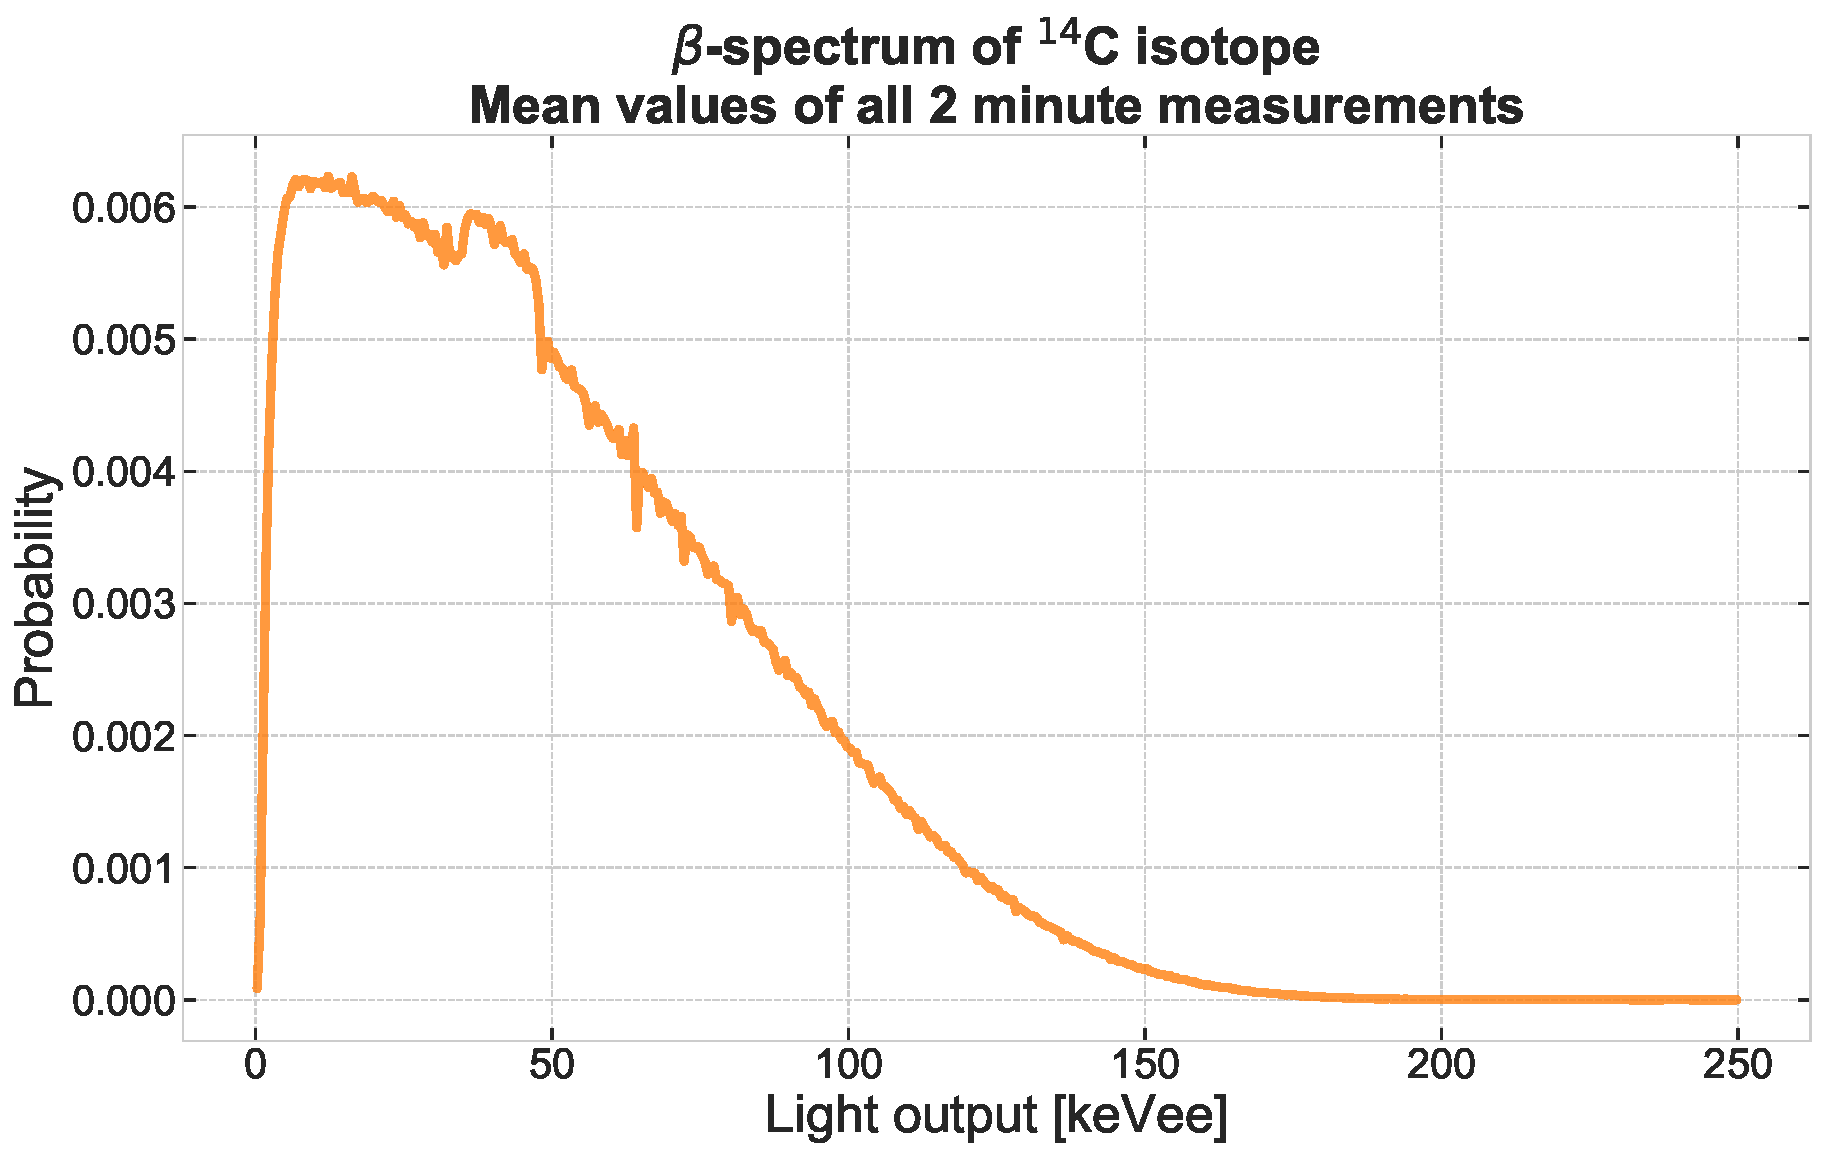
\includegraphics[width=\textwidth]{mean_spectrum.pdf}
    \captionof{figure}{Az általunk vizsgált $^{14}$C különböző, egymás utáni 2 perces mérésekből származó $\beta$-spektrumainak átlagolt értéke.} \label{fig:2}
\end{center}
\vspace*{\fill}
\newpage
\topskip0pt
\vspace*{\fill}
\begin{center}
    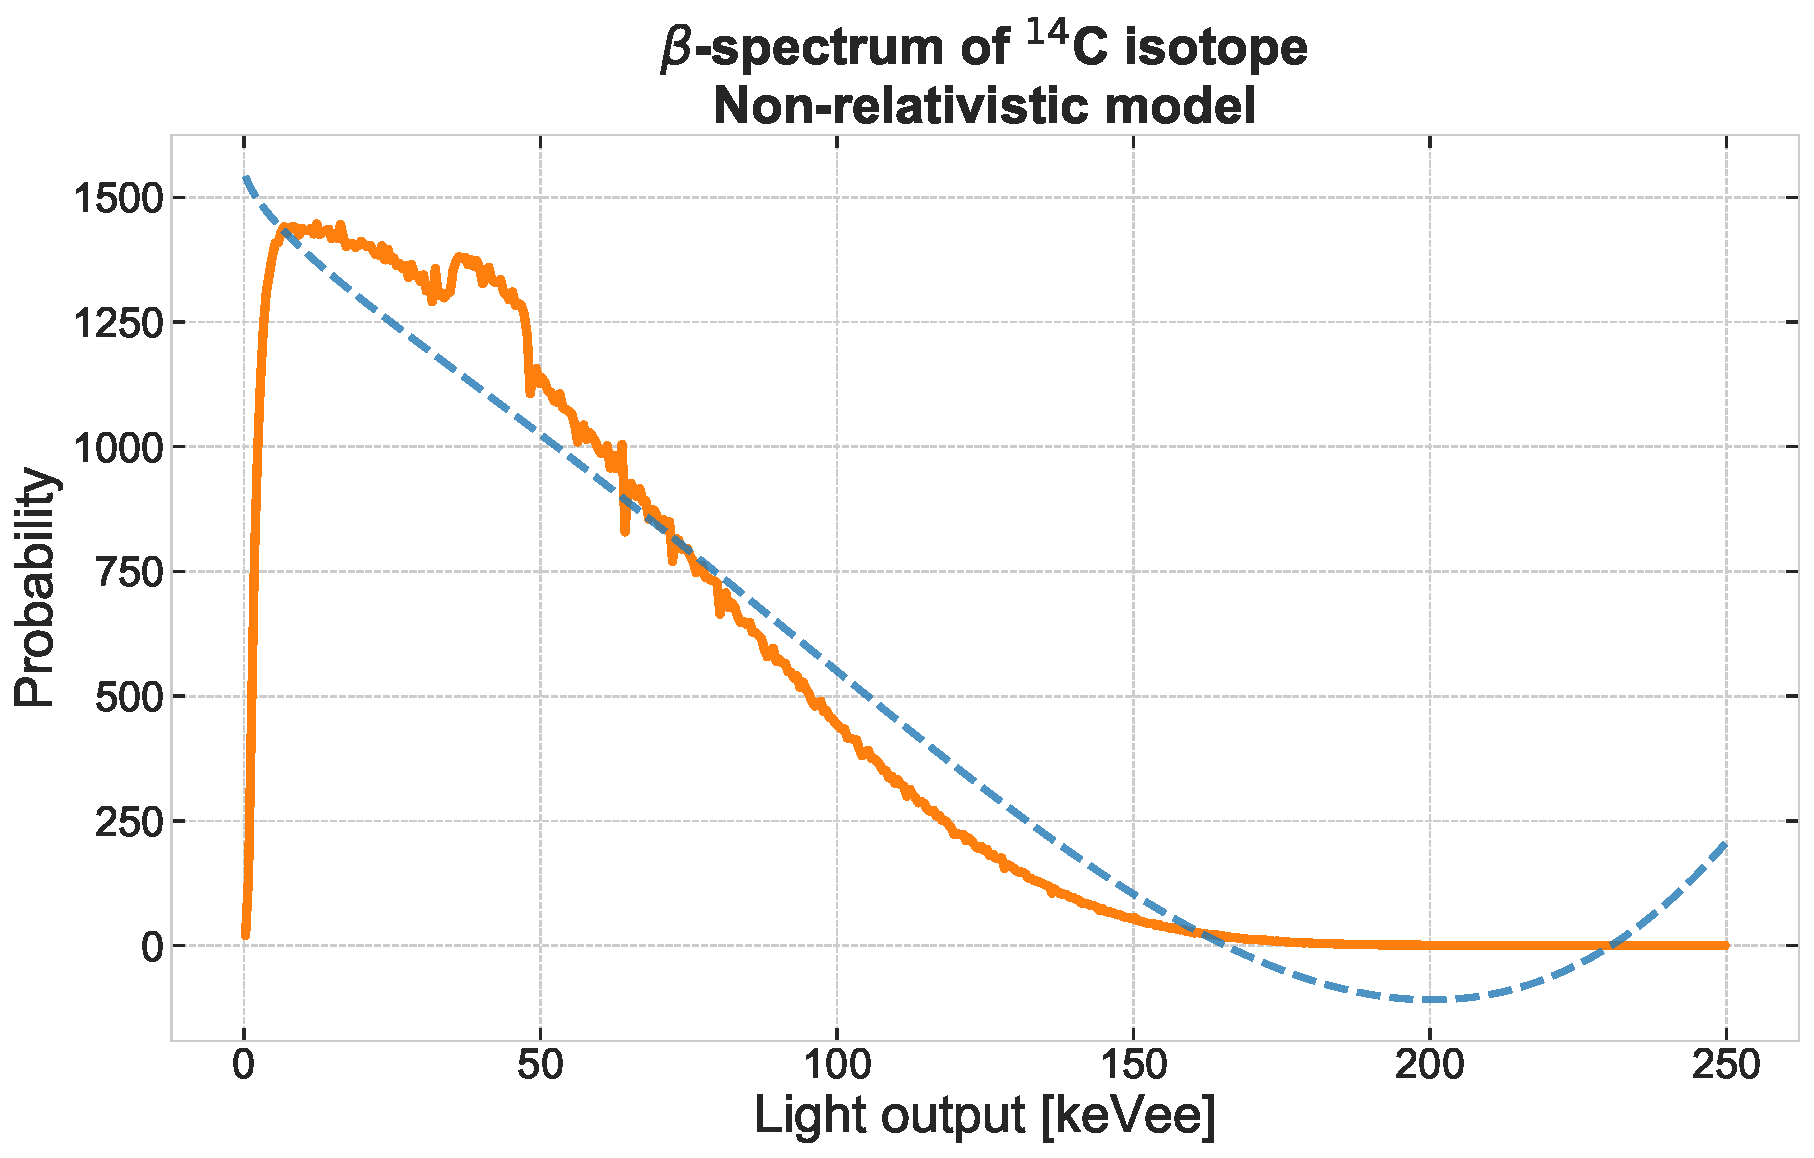
\includegraphics[width=\textwidth]{non_relat_fit.pdf}
    \captionof{figure}{Az általunk vizsgált $^{14}$C kiátlagolt spektrumára illesztett nem-relativisztikus függvény, mely egy túl jó közelítésben, de láthatóan visszaadja a $\beta$-spektrum lecsengő mivoltát. Zérushelye a $^{14}$C karakterisztikus $156.5$ keV-es $Q$ értéke körül van.} \label{fig:3}
\end{center}
\begin{center}
    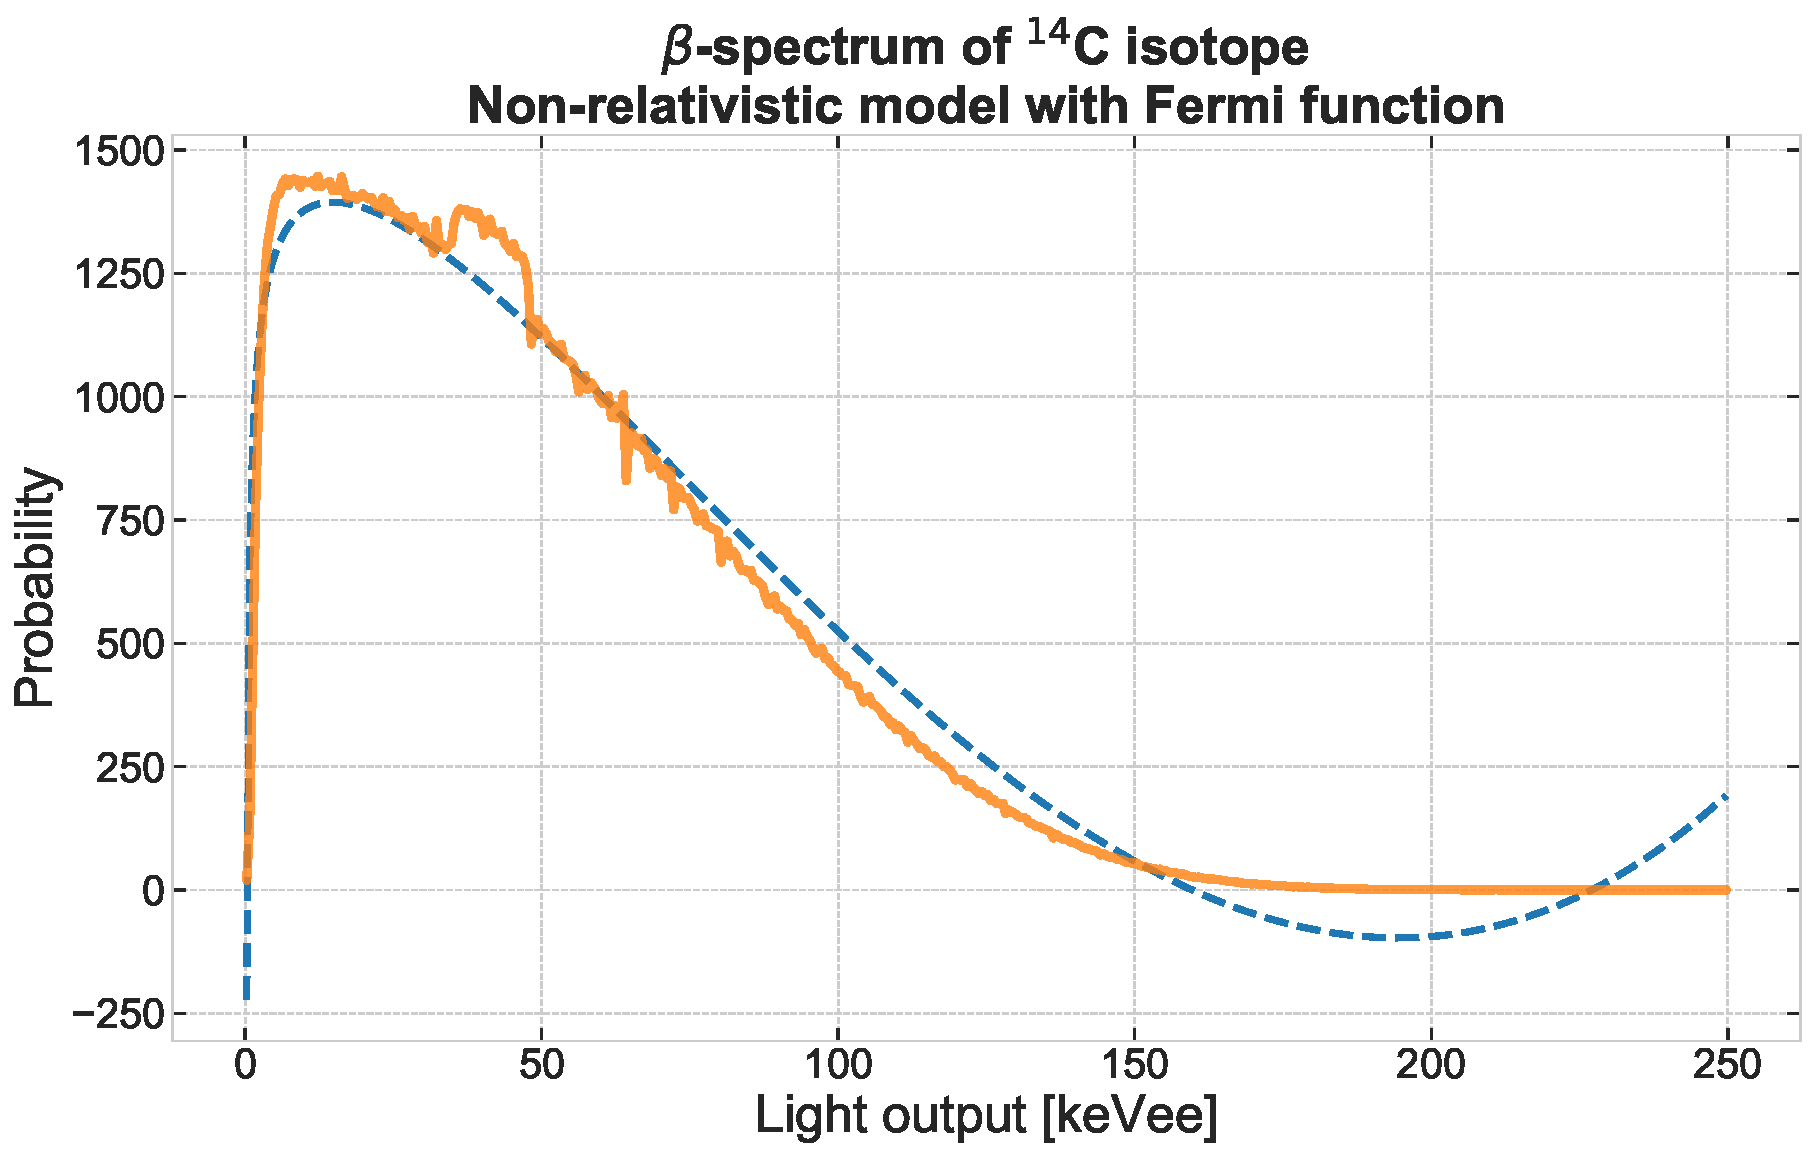
\includegraphics[width=\textwidth]{non_relat_fermi_fit.pdf}
    \captionof{figure}{Az általunk vizsgált $^{14}$C kiátlagolt spektrumára illesztett nem-relativisztikus függvény, mely a Fermi-függvény által nyújtott korrekciót felhasználva, az előzőnél sokkal jobban megközelíti a $\beta$-spektrum görbéjét. A zérushely itt is a $^{14}$C karakterisztikus $156.5$ keV-es $Q$ érték körül van.} \label{fig:4}
\end{center}
\vspace*{\fill}